\section{Aufbau und Durchführung}
\label{sec:auf_durch}

Im Folgenden wird der Aufbau und die Durchführung des Versuchs beschrieben.

\subsection{Der Aufbau}
\label{sec:aufbau}

Die Materialien für den Versuch sind in Abbildung \ref{fig:material} zu sehen. Für den Versuch stehen in einem Baukasten kugelförmige Hohlraumresonatoren als Halbkugeln mit Lautsprecher und Mikrofon jeweils in einer der beiden Hälften zur Verfügung. Außerdem gibt es 2 weitere Halbkugeln mit einem Loch und dazugehörige Blenden mit den Durchmessern von $d = \{ 10, 13, 16 \} \, \mathrm{mm}$. Zusätzlich sind in einem Baukasten zylinderförmige Hohlraumresonatoren mit den Längen von $l = \{62.5,37.5, 50, 75\} \, \mathrm{mm}$ und Blenden mit den Durchmessern von $d = \{ 10, 13, 16 \} \, \mathrm{mm}$ vorhanden. Diese Bauteile können auf eine Schiene aufgebracht werden, wo dann auch ein Lautsprecher und ein Mikrofon als Enden vorhanden sind. Die Messung kann einerseits über einen Computer mit der Software namens \textit{SpectrumSLC} durchgeführt werden. Dabei bietet die Schnittstelle mit dem Computer ein Audiosignal an den Lautsprecher und kann die Signale des Mikrofons empfangen und verarbeiten. Eine andere Variante ist die Messung mit Hilfe eines Oszilloskops. Die Schaltung ist in Abbildung \ref{fig:schaltung} skizziert. Dafür wird der Lautsprecher an der Steuerelektronik an \textit{Speaker Out} und das Mikrofon an \textit{Micro Input} angeschlossen. Ein Sinusgenerator wird einerseits mit Channel 1 vom Oszilloskop verbunden als auch in \textit{Sine Input} der Steuerelektronik. Channel 2 wird an den Anschluss namens \textit{AC Monitor} in der Steuerelektronik angeschlossen. In der Steuerelektronik ist ein Frequenz-Amplitude-Konverter vorhanden, damit die Frequenzen am Oszilloskop untersucht werden können. Mit Hilfe der sweep-Funktion des Sinusgenerators können dann die Daten zeitlich mit der Frequenz am Oszilloskop verarbeitet werden. Am PC können die Daten direkt gespeichert werden und am Oszilloskop können durch Anschließen eines USB-Sticks die Bilder gespeichert werden.

\begin{figure}[H]
    \centering
    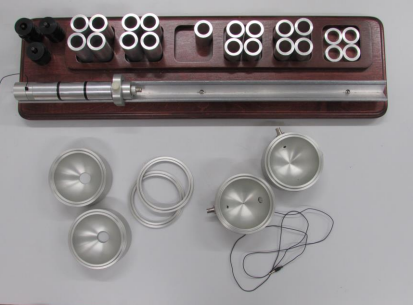
\includegraphics[width=0.8\textwidth]{Experiment.PNG}
    \caption{Hohlraumresonatoren und Aluminiumzylinder. \cite{Anleitung}}
    \label{fig:material}
\end{figure}

\begin{figure}[H]
    \centering
    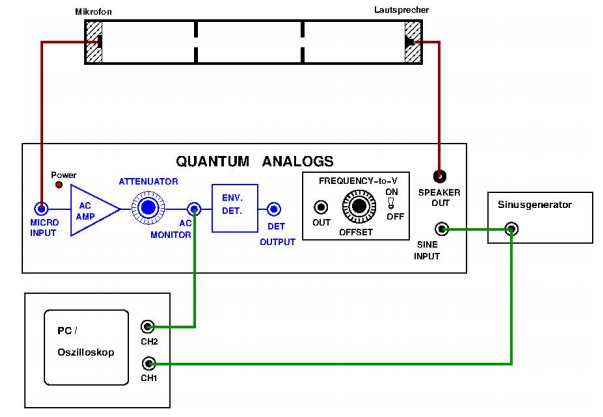
\includegraphics[width=0.8\textwidth]{Schaltung.PNG}
    \caption{Skizze der Schaltung des Versuchs. \cite{Anleitung}}
    \label{fig:schaltung}
\end{figure}

\subsection{Vorbereitende Experimente}
\label{sec:vorbereitung}

Bevor mit den richtigen Experimenten angefangen werden kann, muss die Versuchstechnik getestet werden. Dafür werden die Zylinder mit einer Länge von $50 \, \mathrm{mm}$ benötigt. Es wird nun zuerst ein Zylinder zwischen Lautsprecher und Mikrofon gestellt und ein Frequenzspektrum von $100 \, \mathrm{Hz}$ bis $12 \, \mathrm{kHz}$ mit dem Oszilloskop aufgenommen und dokumentiert. Danach wird ein Zylinder an die Kette angehangen und dasselbe Spektrum aufgenommen. Dies wird bis zum 12. Zylinder durchgeführt. Danach wird dieselbe Messung mit dem Computer durchgeführt. Die Frequenzspektren sollten jeweils keine signifikanten Unterschiede zwischen der Messung mit dem Oszilloskopund dem Computer aufweisen. Zum Schluss wird ein Frequenzspektrum eines einzelnen $75 \, \mathrm{mm}$ Zylinders mit Oszilloskop und Computer aufgenommen und verglichen.

\subsection{Das Wasserstoffatom}
\label{sec:d_H}

Für das Wasserstoffatom wird das Frequenzspektrum eines kugelförimgen Hohlraumresonators mit dem Computer aufgenommen. Die beiden Kugelhälften werden zu einer Kugel zusammengefügt und das Mikrofon und der Lautsprecher sind im Inneren mit einem Winkel von $\alpha = 180°$ ausgerichtet. Das Frequenzspektrum wird in $5 \, \mathrm{Hz}$ Schritten und einer Schrittdauer von $5 \, \mathrm{ms}$ aufgenommen. \newline

Im Anschluss wird wieder das Oszilloskop verwendet und es wird mit einem Sinusgenerator der Frequenzbereich von $100 \, \mathrm{Hz}$ bis $10 \, \mathrm{kHz}$ durchlaufen. Dabei sollte die Frequenz, Amplitude und Phasenverschiebung beobachtet werden. Die auftreteten Resonanzfrequenzen und ihre Ordnung werden dokumentiert. \newline

Im Folgenden wird wieder der Computer verwendet. Ziel ist es für mindestens 4 Resonanzfrequenzen die Druckamplitude als Funktion des Drehwinkels $\alpha$ zu bestimmen. Dafür wird wieder ein Frequenzbereich von $100 \, \mathrm{Hz}$ bis $10 \, \mathrm{kHz}$ durchlaufen mit $5 \, \mathrm{Hz}$ Schritten und einer Schrittdauer von $5 \, \mathrm{ms}$. Dabei wird nach jeder Messung der Winkel $\alpha$ zwischen Mikrofon und Lautsprecher durch Rotation der oberen Kugelhälfte zwischen $0°$ und $180°$ in $10°$ Schritten varriert. \newline

Anschließend werden die Peaks mit verscheidenen Zwischenringen zwischen den Kugelhälften aufgespalten. Dafür wird zuerst zwischen den Kugelhälften jeweils ein Zwischenring mit gesetzt und die Resonanzfrequenz bei ca. $2, \! 3 \, \mathrm{kHz}$ mit $\alpha = 180°$ vermessen. Dafür wird mit dem PC ein hochaufgelöstes Frequenzspektrum zwischen $1, \! 8 \, \mathrm{kHz}$ und $2, \! 6 \, \mathrm{kHz}$ mit $1 \, \mathrm{Hz}$ Schritten und einer Schrittdauer von $5 \, \mathrm{ms}$ aufgenommen. Diese Messung wird für jeden Zwischenring mit jeweils verscheidenem Durchmesser wiederholt. In diesem Experiment werden Zwischenringe mit den Durchmessern von $d = \{ 3, 6, 9 \} \, \mathrm{mm}$ verwendet. \newline

Zum Schluss wird nur der Zwischenring mit $9 \, \mathrm{mm}$ Durchmesser und der Computer verwendet. Dazu wird wie im vorherigen Absatz ein hochaufgelöstes Frequenzspektrum zwischen $1, \! 8 \, \mathrm{kHz}$ und $2, \! 6 \, \mathrm{kHz}$ mit den selben Schrittweiten und -dauern aufgenommen nur für verschiedene Winkel $\alpha$. Dafür wird wieder nach jeder Messung der Winkel $\alpha$ zwischen $0°$ und $180°$ in $10°$ Schritten varriert.

\subsection{Das Wasserstoffmolekül}
\label{sec:d_H2}

Für das Wasserstoffmolekül wird zwischen den Kugelhälften mit Mirkorfon und Lautsprecher 2 Hälften mit einem Loch gesetzt, sodass 2 Kugelresonatoren entstehen, die durch eine Öffnung verbunden sind. Im Anschluss wird jeweils mit dem Computer ein hochaufgelöstes Frequenzspektrum zwischen $2, \! 2 \, \mathrm{kHz}$ und $2, \! 5 \, \mathrm{kHz}$ mit $1 \, \mathrm{Hz}$ Schritten und einer Schrittdauer von $7, \! 5 \, \mathrm{ms}$ aufgenommen. Dies wird für verschiedene Blenden mit unterschiedlichen Durchmessern zwischen den Kugelresonatoren wiederholt. Im Experiment sind Blenden mit den Durchmessern von $d = \{ 5, 10, 15, 20 \} \, \mathrm{mm}$ vorhanden. \newline

Danach wird nur die $20 \, \mathrm{mm}$ Blende und der Computer verwendet. Jetzt wird wieder ein hochaufgelöstes Frequenzspektrum zwischen $2, \! 2 \, \mathrm{kHz}$ und $2, \! 5 \, \mathrm{kHz}$ mit $1 \, \mathrm{Hz}$ Schritten und einer Schrittdauer von $7, \! 5 \, \mathrm{ms}$ aufgenommen und dies wird für jeden Winkel $\alpha$ in $10°$ Schritten zwischen $0°$ und $180°$ wiederholt.

\subsection{Der 1-dim Festkörper}
\label{sec:d_fk}

Der 1 dimensionale Festkörper wird in diesem Experiment durch eine Resonatorkette aus Aluminiumzylindern und Irisblenden simuliert. Am Anfang und Ende befindet sich der Lautsprecher und das Mikrofon. Zur Verfügung stehen Zylinder der Längen $l = \{ 62.5, 37.5, 50, 75 \} \, \mathrm{mm}$ und Irisblenden mit den Durchmessern von $d = \{ 10, 13, 16 \} \, \mathrm{mm}$. In diesem Teil des Experiment werden mit dem Computer immer Frequenzspektren von $100 \, \mathrm{Hz}$ bis $12 \, \mathrm{kHz}$ und $5 \, \mathrm{Hz}$ Schritten mit einer Schrittdauer von $50 \, \mathrm{ms}$ aufgenommen. \newline

Zu Beginn werden 2 Zylinder mit $50 \, \mathrm{mm}$ Länge und einer $16 \, \mathrm{mm}$ Blende dazwischen zu einer Kette zusammengefügt und das Frequenzspektrum wird aufgenommen. Nach der Messung wird die Kette um einen Zylinder und eine Blende mit der selben Länge und Durchmesser ergäntzt und dieselbe Messung wiederholt. Dies wird wiederholt bis zu einer Länge von 10 Zylindern. \newline

Dieses Experiment wird nun wiederholt mit einer Kette aus jeweils 2, 4 und 10 Zylindern. Der einzige Unterschied ist nun, dass dies mit Blenden mit $13 \, \mathrm{mm}$ und $10 \, \mathrm{mm}$ Durchmesser jeweils durchgeführt wird. \newline

Im Anschluss werden wieder Blenden mit $16 \, \mathrm{mm}$ Durchmesser verwendet. In der Kette aus 10 Zylindern wird nun einer der $50 \, \mathrm{mm}$ Zylinder durch einen Zylinder mit $75 \, \mathrm{mm}$ ausgetauscht und das selbe Frequenzspektrum gemessen. Danach wird der $75 \, \mathrm{mm}$ Zylinder durch 3 Zylinder mit $62, \! 5 \, \mathrm{mm}$ Länge, die zusammen dann einen $37, \! 5 \, \mathrm{mm}$ langen Zylinder ergeben, ausgetauscht und wieder das Frequenzspektrum aufgenommen. Dann werden diese 3 Zylinder durch einen $50 \, \mathrm{mm}$ und einen $12, \! 5 \, \mathrm{mm}$ Zylinder ersetzt, die dann zusammen einen $62, \! 5 \, \mathrm{mm}$ langen Zylinder ergeben und wieder wird das Frequenzspektrum aufgenommen. \newline

Nun wird eine Kette aus 10 Zylindern zusammengebaut, bei denen jeweils abwechselnd ein $50 \, \mathrm{mm}$ Zylinder und ein $75 \, \mathrm{mm}$ Zylinder eingebaut wird mit einer $16 \, \mathrm{mm}$ Blenden immer dazwischen. Wieder wird das Frequenzspektrum aufgenommen. \newline

Zum Schluss wird eine Kette aus 8 Zylindern mit einer Länge von $50 \, \mathrm{mm}$ zusammengebaut. Dabei besitzt jede Blende zwischenden Zylindern abwechselndeinen Durch messer von $13 \, \mathrm{mm}$ und $16 \, \mathrm{mm}$. Dann wird das Frequenzspektrum aufgenommen.
